% !TeX spellcheck = de_DE
\documentclass{uebung_cs}
\usepackage{algo121}
\blattname{Wochenplan: Disjunkte Mengen, Union-Find}

%%%%%%%%%%%%%%%%%%%%%%%%%%%%%%%%%%%%%%%%%%%%%%%%%%%%%%%%%%%%%%%%%%%%%%%%%%%%

\newboolean{programming}
\setboolean{programming}{false}

%%%%%%%%%%%%%%%%%%%%%%%%%%%%%%%%%%%%%%%%%%%%%%%%%%%%%%%%%%%%%%%%%%%%%%%%%%%%
% Makros für noch nicht übersetzte Begrifflichkeiten
\newcommand{\qfind}{\textit{\textbf{Quick Find}}}
\newcommand{\qunion}{\textit{\textbf{Quick Union}}}
\newcommand{\wqunion}{\textit{\textbf{Weighted Quick Union}}}
\newcommand{\pathcomp}{\textit{\textbf{Path Compression}}}


\begin{document}
\section*{Vorbereitung}
Lies CLRS Kapitel 21 ohne 21.4 (oder Algorithms 4ed. Kapitel 1.5) und schau das Video der Woche.

\section*{Dienstag}
\begin{aufgabe}[Union Find von Hand laufen lassen]\label{tue-first}
	Sieh dir die folgende Sequenz an Operationen an:
	\texttt{Init(7), Union(3,4),  Union(5,0), Union(4,5), Union(4,3), Union(0,1), Union(2,6), Union(0,4)} und \texttt{Union(6,0)}
	\begin{enumerate}
		\item (\warmup) Führe die Sequenz mittels \qfind von Hand durch.
		Zeige, wie die Inhalte des $id$ Feldes nach jedem Schritt aussehen.
		Die \texttt{Union($i,j$)} Operation aktualisiert hierbei immer $id$ für die Menge, die durch $i$ gegeben wird.
		\item (\warmup) Führe die Sequenz mittels \qunion von Hand durch.
		Zeige, wie der Baum nach jedem Schritt aussehen.
		Die \texttt{Union($i,j$)} Operation setzt hierbei immer die Wurzel von Baum von $i$ als ein Kind der Wurzel des Baumes von $j$.
		\item Führe die Sequenz mittels \wqunion von Hand durch.
		Zeige, wie der Baum nach jedem Schritt aussehen.
		Die \texttt{Union($i,j$)} Operation setzt hierbei immer die Wurzel von Baum von $i$ als ein Kind der Wurzel des Baumes von $j$, wenn die Größe der beiden Bäume gleich ist.
		\item Zeige das Resultat von \pathcomp auf einem der Bäume aus a) und b) nach einer \texttt{Find($x$)} Operation, für die Fälle, dass $x$ ein Blatt ist, $x$ ein innerer Knoten mit Tiefe 1 ist oder $x$ ein innerer Knoten mit Höhe 1 ist 
	\end{enumerate}
\end{aufgabe}

\begin{aufgabe}[Alternative zum \qfind Algorithmus]
	Eine Kommilitonin stellt die folgende, intuitive Variante von \qfind \texttt{Union} vor.
	Funktioniert sie?
	\begin{algorithmic}
		\STATE \texttt{Union}(i,j)
		\IF{\texttt{Find}($i$) $\neq$ \texttt{Find}($j$)}
			\FOR{$k = 0$ \textbf{to} $n - 1$}
				\IF{$id[k] == id[i]$}
					\STATE $id[k] = id[j]$
				\ENDIF
			\ENDFOR
		\ENDIF
	\end{algorithmic}
\end{aufgabe}

\begin{aufgabe}[Dynamische Zusammenhangskomponente und Suche in Graphen]
	Mittels Tiefen- und Breitensuche können wir die Zusammenhangskomponente eines Graphs finden.
	Entwirf eine einfache Lösung für die dynamische Zusammenhangskomponente mittels Suche in Graphen und vergleichedie Komplexität deiner Lösung mit der auf Union-Find basierenden Lösung.
\end{aufgabe}

\ifthenelse{\boolean{programming}}{
\begin{aufgabe}[Implememtierung von Union-Find]
	Wir wollen Datenstrukturen für Union-Find in einer beliebigen Programmiersprache implementieren, die \texttt{Init}, \texttt{Union} und \texttt{Find} unterstützen.
	\begin{enumerate}
		\item Implementiere \qunion
		\item Erweitere deine Implementierung mit \wqunion
		\item Erweitere deine Implementierung mit \pathcomp
	\end{enumerate}
\end{aufgabe}
}{}

\begin{aufgabe}[Zombie Invasion, \hard]
	In der post-apokalyptischen Zukunft (ein unaufmerksamer Student hat bei Zombieduel-Experimenten versehentlich einige freigelassen) haben du und eine kleine Gruppe an Überlebenden sich in einem kleinen Gebäude verbarrikadiert.
	Das einzige was zwischen euch und einer hungrigen Horde Zombies steht ist ein Grid von $k\times k$ Wänden.\\\\
	\begin{center}
		\newcommand{\wallAt}[2]{
			% draws 1x0.6 wall at (#1,#2)
			\draw[fill=black!25,draw=none] (#1-0.45,#2*0.7+0.3) rectangle (#1+0.45,#2*0.7-0.3);
		}
		\begin{tikzpicture}
			% draw each layer
			\foreach \x in {0,1,2,4}{
				\wallAt{\x}{0}
			}
			\foreach \x in {0,2,4,5}{
				\wallAt{\x}{1}
			}
			\foreach \x in {1,2,3,4,5}{
				\wallAt{\x}{2}
			}
			\foreach \x in {2,5}{
				\wallAt{\x}{3}
			}
			\foreach \x in {1,2,4,5}{
				\wallAt{\x}{4}
			}
			\foreach \x in {1,2,3,4,5}{
				\wallAt{\x}{5}
			}
			% draw delimiters
			\draw[line width=2pt] (-0.7,5*0.7 + 1) -- (-0.7,-1);
			\draw[line width=2pt] (5.7,5*0.7 + 1) -- (5.7,-1);
		\end{tikzpicture}
		\hspace{0.7cm}
		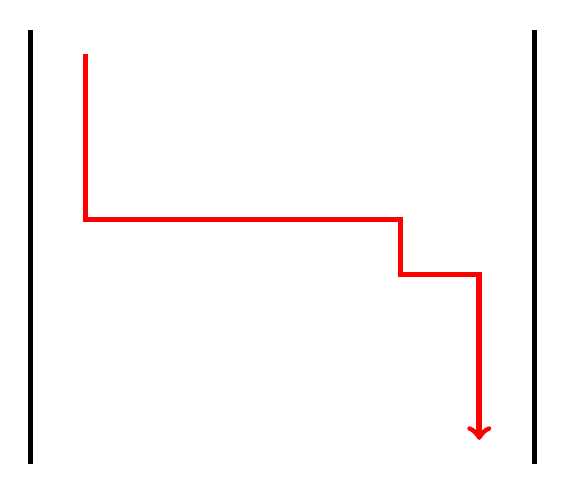
\begin{tikzpicture}
			% draw each layer
			\foreach \x in {0,1,2,4}{
				\wallAt{\x}{0}
			}
			\foreach \x in {2,4}{
				\wallAt{\x}{1}
			}
			\foreach \x in {1,2,3}{
				\wallAt{\x}{2}
			}
			\foreach \x in {5}{
				\wallAt{\x}{3}
			}
			\foreach \x in {1,2,5}{
				\wallAt{\x}{4}
			}
			\foreach \x in {1,3,4}{
				\wallAt{\x}{5}
			}
			% draw delimiters
			\draw[line width=2pt] (-0.7,5*0.7 + 1) -- (-0.7,-1);
			\draw[line width=2pt] (5.7,5*0.7 + 1) -- (5.7,-1);
			% zombie path
			\draw[->, line width=2pt, red] (0, 6*0.7) -- (0,3*0.7) -- (4,3*0.7) -- (4,2*0.7) -- (5,2*0.7) -- (5,-0.7); 
		\end{tikzpicture}
	\end{center}
	Oberhalb des Grids warten die Zombies, während deine Gruppe und du unterhalb sind.
	Unglücklicherweise sind die Wände alt und spröde und stürzen regelmäßig ein.
	Sobald ein Pfad von ganz oben nach ganz unten verläuft kommen die Zombies durch.
	Um eure Evakuierung vorzubereiten willst du permanent überprüfen, ob es einen entsprechenden Pfad durch das Grid gibt.
	Entwirf eine Datenstruktur, die es effizient den Überblick behält, während die Wände (Zellen des Grids) eine nach der anderen einstürzen.
\end{aufgabe}

\begin{aufgabe}[Rekursive \pathcomp, \hard]
	Entwirf eine rekursive Variante von \pathcomp in Pseudo-Code.
\end{aufgabe}

\begin{aufgabe}[Union-Find mit verketteten Listen und Gewichtungen]
	Wir wollen eine Variante von \qfind mittels verketteten Listen auf die folgende Art und Weise implementieren.
	Jede Menge wird durch eine einfach verkettete Liste repräsentiert.
	Der Repräsentant jeder Menge ist das erste Element der respektiven Liste und jedes Element der Liste hat einen Pointer auf den Repräsentanten.
	Des weiteren haben wir einen Pointer \textit{tail} auf das letzte Element der Liste.
	Zum Beispiel eine Datenstruktur für die Menge $\{1,4,7,8,14\}$ mit Repräsentant $7$ könnte wie folgt aussehen:
	\begin{center}
		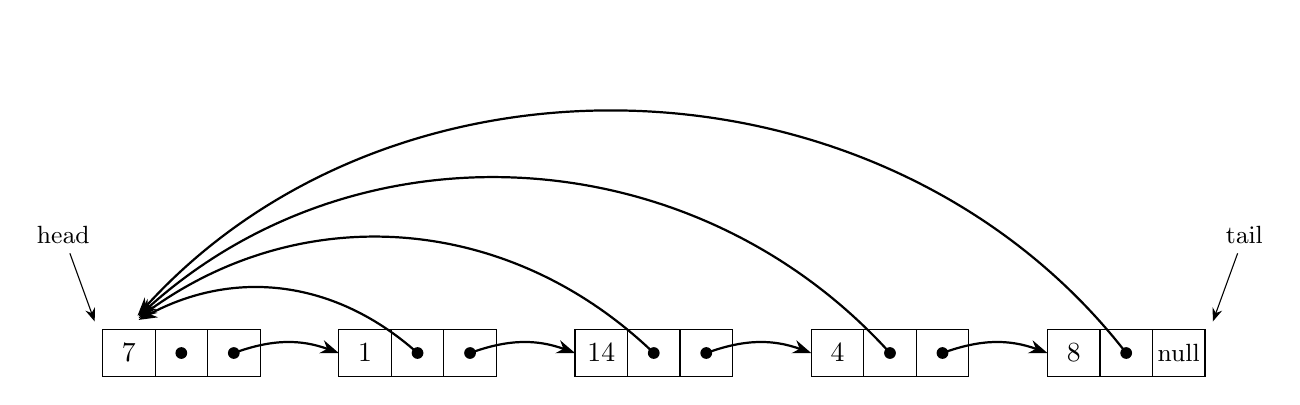
\begin{tikzpicture}
			\usetikzlibrary{arrows.meta}
			\newcommand{\listElem}[4]{  
				% draws list elements 
				% args: 
				%     "rank" (ordered left to right)
				%     label
				%     fill color for base circle of next pointer
				%     text at next pointer slot
				\draw (#1*3, 0.3) rectangle (#1*3 + 2,-0.3);
				\draw (#1*3 + 2/3, 0.3) -- (#1*3 + 2/3, -0.3);
				\draw (#1*3 + 4/3, 0.3) -- (#1*3 + 4/3, -0.3);
				\node (val_#2) at (#1*3 + 1/3, 0) {#2};
				\node (top_#2) at (#1*3 + 1/3, 0.35) {};
				\node (left_#2) at (#1*3, 0) {};
				\node[fill=black, circle, inner sep=1.5pt] (repr_#2) at (#1*3 + 1, 0) {};
				\node[fill=#3, circle, inner sep=1.5pt] (nxt_#2) at (#1*3 + 5/3, 0) {};
				\node () at (nxt_#2) {\small #4};
			}
			\newcommand{\listReprPtr}[3]{
				% args:
				%     from label
				%     to label
				%     bend angle
				\draw[-Stealth, thick] (repr_#1.center) to [bend right=#3] (top_#2);
			}
			\newcommand{\listNxtPtr}[3]{
				% args:
				%     from label
				%     to label
				%     bend angle
				\draw[-Stealth, thick] (nxt_#1.center) to [bend left=#3] (left_#2.center);
			}
			% wrappers
			\newcommand{\regularListElem}[2]{ \listElem{#1}{#2}{black}{} }
			\newcommand{\tailListElem}[2]{ \listElem{#1}{#2}{white}{null} }
			%
			% draw the list
			% elements of the list
			\regularListElem{0}{7}
			\regularListElem{1}{1}
			\regularListElem{2}{14}
			\regularListElem{3}{4}
			\tailListElem{4}{8}
			% representative pointers
			% aufsteigende grade sorgen dafür, dass die pfeilspitzen nicht
			% alle exakt im selben punkt landen
			\listReprPtr{1}{7}{35}
			\listReprPtr{14}{7}{40}
			\listReprPtr{4}{7}{45}
			\listReprPtr{8}{7}{50}
			% next pointers
			\listNxtPtr{7}{1}{20}
			\listNxtPtr{1}{14}{20}
			\listNxtPtr{14}{4}{20}
			\listNxtPtr{4}{8}{20}
			% head ptr, tail ptr
			\node (headptr) at (-0.5, 1.5) {\small head};
			\node (tailptr) at (14.5, 1.5) {\small tail};
			\draw[-Stealth] (headptr) -- (-0.1, 0.4);
			\draw[-Stealth] (tailptr) -- (14.1, 0.4);
		\end{tikzpicture}
	\end{center}
	\begin{enumerate}
		\item Zeige, unter Benutzung der Repräsentation, wie \texttt{Init($n$)} in Zeit $O(n)$, \texttt{Find($i$)} in Zeit $O(1)$ und \texttt{Union($i,j$)} in Zeit $O(|S(i)|)$, wobei $S(i)$ die Menge mit $i$ ist.
		\item Zeige, wie man die Lösung erweitern kann, sodass \texttt{Init} und \texttt{Find} dieselbe Zeitkomplexität haben, aber \texttt{Union($i,j$)} in Zeit $O(\min(|S(i)|, |S(j)|))$ benötigt.\\
		\textit{Hinweis: Speichere ein paar Zusatzinformationen}
		\item (\hard) Zeige, dass für $p$ \texttt{Find} und $m$ \texttt{Union} Operationen auf $n$ Elementen die zuvorige Lösung eine Laufzeit in $O(p + m\log n)$ benötigt.
	\end{enumerate}
\end{aufgabe}


\end{document}
